\chapter{Evaluation}
How do we evaluate the Solution?\newline
  By measuring the overall throughput and comparing the scenarios\newline
\section{Test arrangement}
What was the test-arrangement? \newline
  \subsection{Physical Infrastructure}
    \begin{figure}[t]
      \centering
      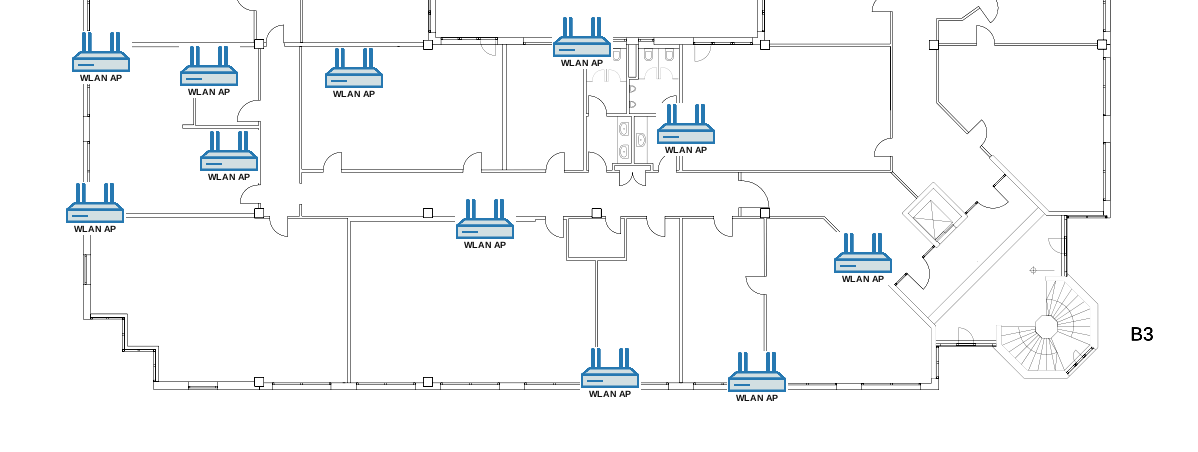
\includegraphics[width=1\columnwidth]{figures/Lancom-flur-withaps}
      \caption{Testsetup deployment: Lancom 2nd floor}
      \label{fig:2ndfloor}
    \end{figure}
    \begin{description}
     \item[Placement of the system?]
     \item[What are the characteristics of the physical environment? (Walls/Interference from other devices/...)]
     \item[Limitations due to physical restrictions]
      Distance between APs maybe not big enough, despite transmission power reduction. Limitations due to cabling\newline
      So the Hidden station Problem not fully visible -> results should be even better compared to base scenario \newline
    \end{description}
  \subsection{Network Infrastructure}
    Image of AutoWDSstatus Topology: (How to place the nodes? What to show?)
    OpenVZ \newline
    VLAN \newline
    IPerf \newline
\section{Metrics}
  \subsection{Durations}
    \begin{description}
     \item[How long were the tests run?]
      10 Minutes
     \item[Measurement Intervalls]
      7 Seconds
    \end{description}
  \subsection{Channelusage}
    Which Channels were used and in what combinations? \newline
      1 \newline
      36 \newline
      1,6,11 \newline
      36,40,44 \newline
      1,6,11,36,40,44 \newline
  \subsection{Characteristics}
    \begin{description}
     \item [When did the tests take place?]
      Mainly Sundays / Holidays in the evening \newline
     \item[Transmission powers used for the tests]
      Antenna gain 3 dB \newline
      Antenna gain 20 dB + Transmitt power reduction \newline
    \end{description}
\section{Results}
  \subsection{Expectations}
    What results would we expect?\newline
  \subsection{Actual Results}
    \begin{description}
     \item [Do the actual results diverge from the expected ones?]
     \item[Assessment of the base scenario]
      Base Scanario (uses only 1 Channel for all connections) pretty much broken by design -> Medium totally overloaded -> does not even scale to 3 APs in close proximity \newline
     \item[By how much is the solution better then before?]
      Despite being actually usable again, Traffic throughput is ~7-10 Times higher
    \end{description}
\section{Reflection on the requirements}
  How far does the solution meet the requirements?\newline
  \subsection{Increased Throughput}
    Definitely, see Diagrams \newline
  \subsection{Reduced Connectivity failures}
    Not tested, since test equippment lacks support for multi-flow/routing support (only bridged connections between APs) \newline
  \subsection{Multiple Radios utilized}
    Surely, with excess radios being usable for client connections \newline
  \subsection{Solution works within the perimeter}
    Absolutely, since we can compute CAA on central entity and works best for static scenarios \newline
  \subsection{Comply with Economic Restrictions}
    Runtime for Small scenarios (about 13 APs with about 500 Possible connections) on a modern system (fill in description of system) small -> <1 Second
    Estimate for bigger scenario missing (How do i correctly estimate that?)
\section{Reflection on related Work}
  Comparison to related Work algorithms\newline
  \subsection{Features of other Systems}
  \subsection{Features of our System}
\section{Discussion}
  \begin{description}
   \item [Checking the coloring and channel assignment after the algo run]
   this might not be the best place for this point, but serves just as a reminder.
   \item [What do the results mean?]
   Obviously it is useful to use mutliple channels for WDS system
   \item[What could'nt we measure?]
   What measurements are still missing:  run testcases for each parameter like formula,...
   Evaluate the redundant paths feature.
  \end{description}